\documentclass{article}

\usepackage{fancyhdr}
\usepackage{extramarks}
\usepackage{minted}
\usepackage{color}
\usepackage[english]{babel}
\usepackage{graphicx}
\graphicspath{ {../assets/} }

%
% Basic Document Settings
%

\topmargin=-0.45in
\evensidemargin=0in
\oddsidemargin=0in
\textwidth=6.5in
\textheight=9.0in
\headsep=0.25in

\linespread{1.1}

\pagestyle{fancy}
\lhead{\hmwkAuthorName}
\chead{\hmwkClass\ (\hmwkClassInstructor): \hmwkTitle}
\rhead{\firstxmark}
\lfoot{\lastxmark}
\cfoot{\thepage}

\renewcommand\headrulewidth{0.4pt}
\renewcommand\footrulewidth{0.4pt}

\setlength\parindent{0pt}
\setlength{\parskip}{1em}

%
% Minted Settings
%

\setminted{frame=lines}
\setminted{linenos}
\setminted{autogobble}

%
% Create Problem Sections
%

\newcommand{\enterProblemHeader}[1]{
    \nobreak\extramarks{}{Assignment \arabic{#1} continued on next page\ldots}\nobreak{}
    \nobreak\extramarks{Assignment \arabic{#1} (continued)}{Assignment \arabic{#1} continued on next page\ldots}\nobreak{}
}

\newcommand{\exitProblemHeader}[1]{
    \nobreak\extramarks{Assignment \arabic{#1} (continued)}{Assignment \arabic{#1} continued on next page\ldots}\nobreak{}
    \stepcounter{#1}
    \nobreak\extramarks{Assignment \arabic{#1}}{}\nobreak{}
}

\setcounter{secnumdepth}{0}
\newcounter{partCounter}
\newcounter{homeworkProblemCounter}
\setcounter{homeworkProblemCounter}{1}
\nobreak\extramarks{Assignment \arabic{homeworkProblemCounter}}{}\nobreak{}

%
% Homework Problem Environment
%
% This environment takes an optional argument. When given, it will adjust the
% problem counter. This is useful for when the problems given for your
% assignment aren't sequential. See the last 3 problems of this template for an
% example.
%
\newenvironment{homeworkProblem}[1][-1]{
    \ifnum#1>0
        \setcounter{homeworkProblemCounter}{#1}
    \fi
    \section{Assignment \arabic{homeworkProblemCounter}}
    \setcounter{partCounter}{1}
    \enterProblemHeader{homeworkProblemCounter}
}{
    \exitProblemHeader{homeworkProblemCounter}
}

%
% Homework Details
%   - Title
%   - Due date
%   - Class
%   - Section/Time
%   - Instructor
%   - Author
%

\newcommand{\hmwkTitle}{Midterm Assignment}
\newcommand{\hmwkDueDate}{March 04, 2019}
\newcommand{\hmwkClass}{CSE 5539}
\newcommand{\hmwkClassInstructor}{Professor Wang}
\newcommand{\hmwkAuthorName}{\textbf{Jeremy Grifski}}

%
% Title Page
%

\title{
    \vspace{2in}
    \textmd{\textbf{\hmwkClass:\ \hmwkTitle}}\\
    \normalsize\vspace{0.1in}\small{Due\ on\ \hmwkDueDate\ at 12:30pm}\\
    \vspace{0.1in}\large{\textit{\hmwkClassInstructor}}
    \vspace{3in}
}

\author{\hmwkAuthorName}
\date{}

\renewcommand{\part}[1]{\textbf{\large Part \Alph{partCounter}}\stepcounter{partCounter}\\}

% Alias for the Solution section header
\newcommand{\solution}{\textbf{\large Solution}}

\begin{document}

\maketitle

\pagebreak

\begin{homeworkProblem}

In this assignment, we were asked to perform pitch detection by correlogram.

On the input side, we were given two files: "ar0.dat" and "er4.dat". These
files contained the result of some signal processing using a bank of gammatone
filters and the Meddis hair cell model. In terms of formatting, each file
contained 64x325 data points. Specifically, the data was organized in order
of 325 time steps. For each time step, there were 64 data points corresponding
to the output of the 64 gammatone filters.

In order to parse the file, I used a combination of MATLAB's load and reshape
functions. These functions allowed me to convert each data file from a stream
to a 64x325 matrix. To be clear, each row contained the entire time series data
for a particular filter.

From there, I generated both a correlogram and a summary correlogram from the
matrix. To do so, I created a correlogram matrix of size 125x64. Naturally,
the 64 corresponds to the channel number and 125 corresponds to the maximum lag.
To populate the correlogram matrix, I iterated over each channel and delay
to accumulate the autocorrelation for the given window. In this case, I had to
perform 200 sums for the 200 step window. The following images are the
resulting correlograms using the first 20 odd-numbered channels:

\begin{figure}[H]
  \caption{The ar0 Correlogram}
  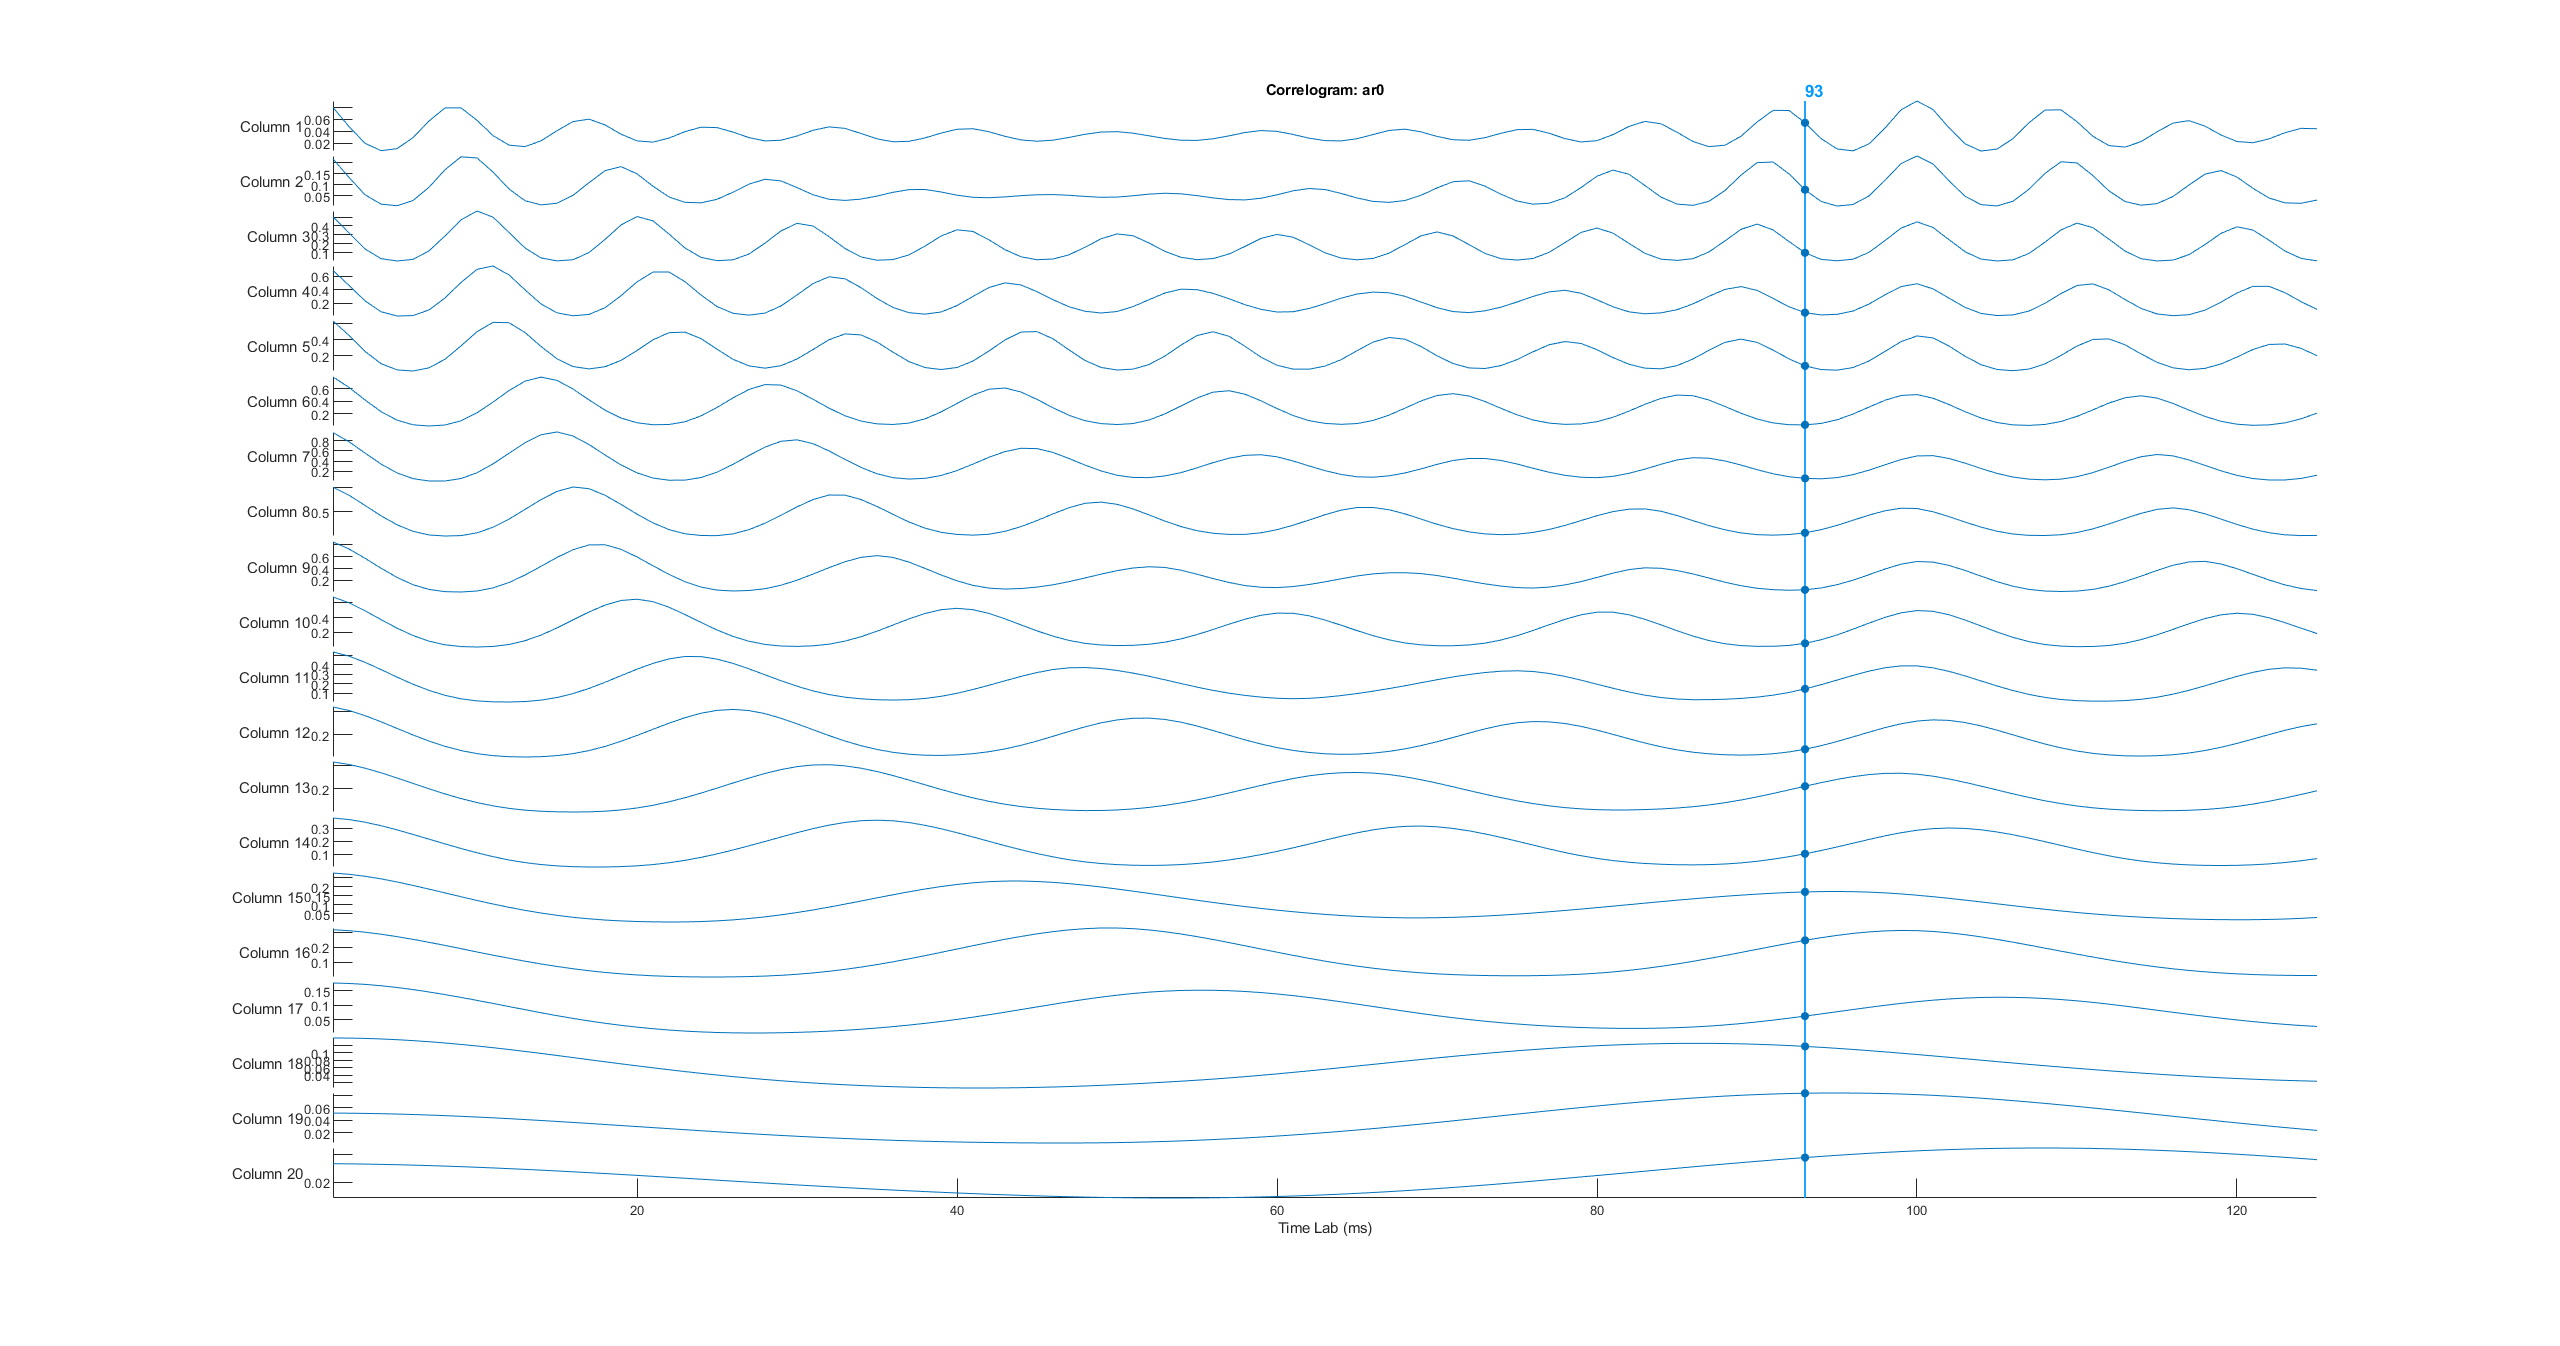
\includegraphics[scale=.25]{ar0-correlogram}
  \centering
\end{figure}

\begin{figure}[H]
  \caption{The er4 Correlogram}
  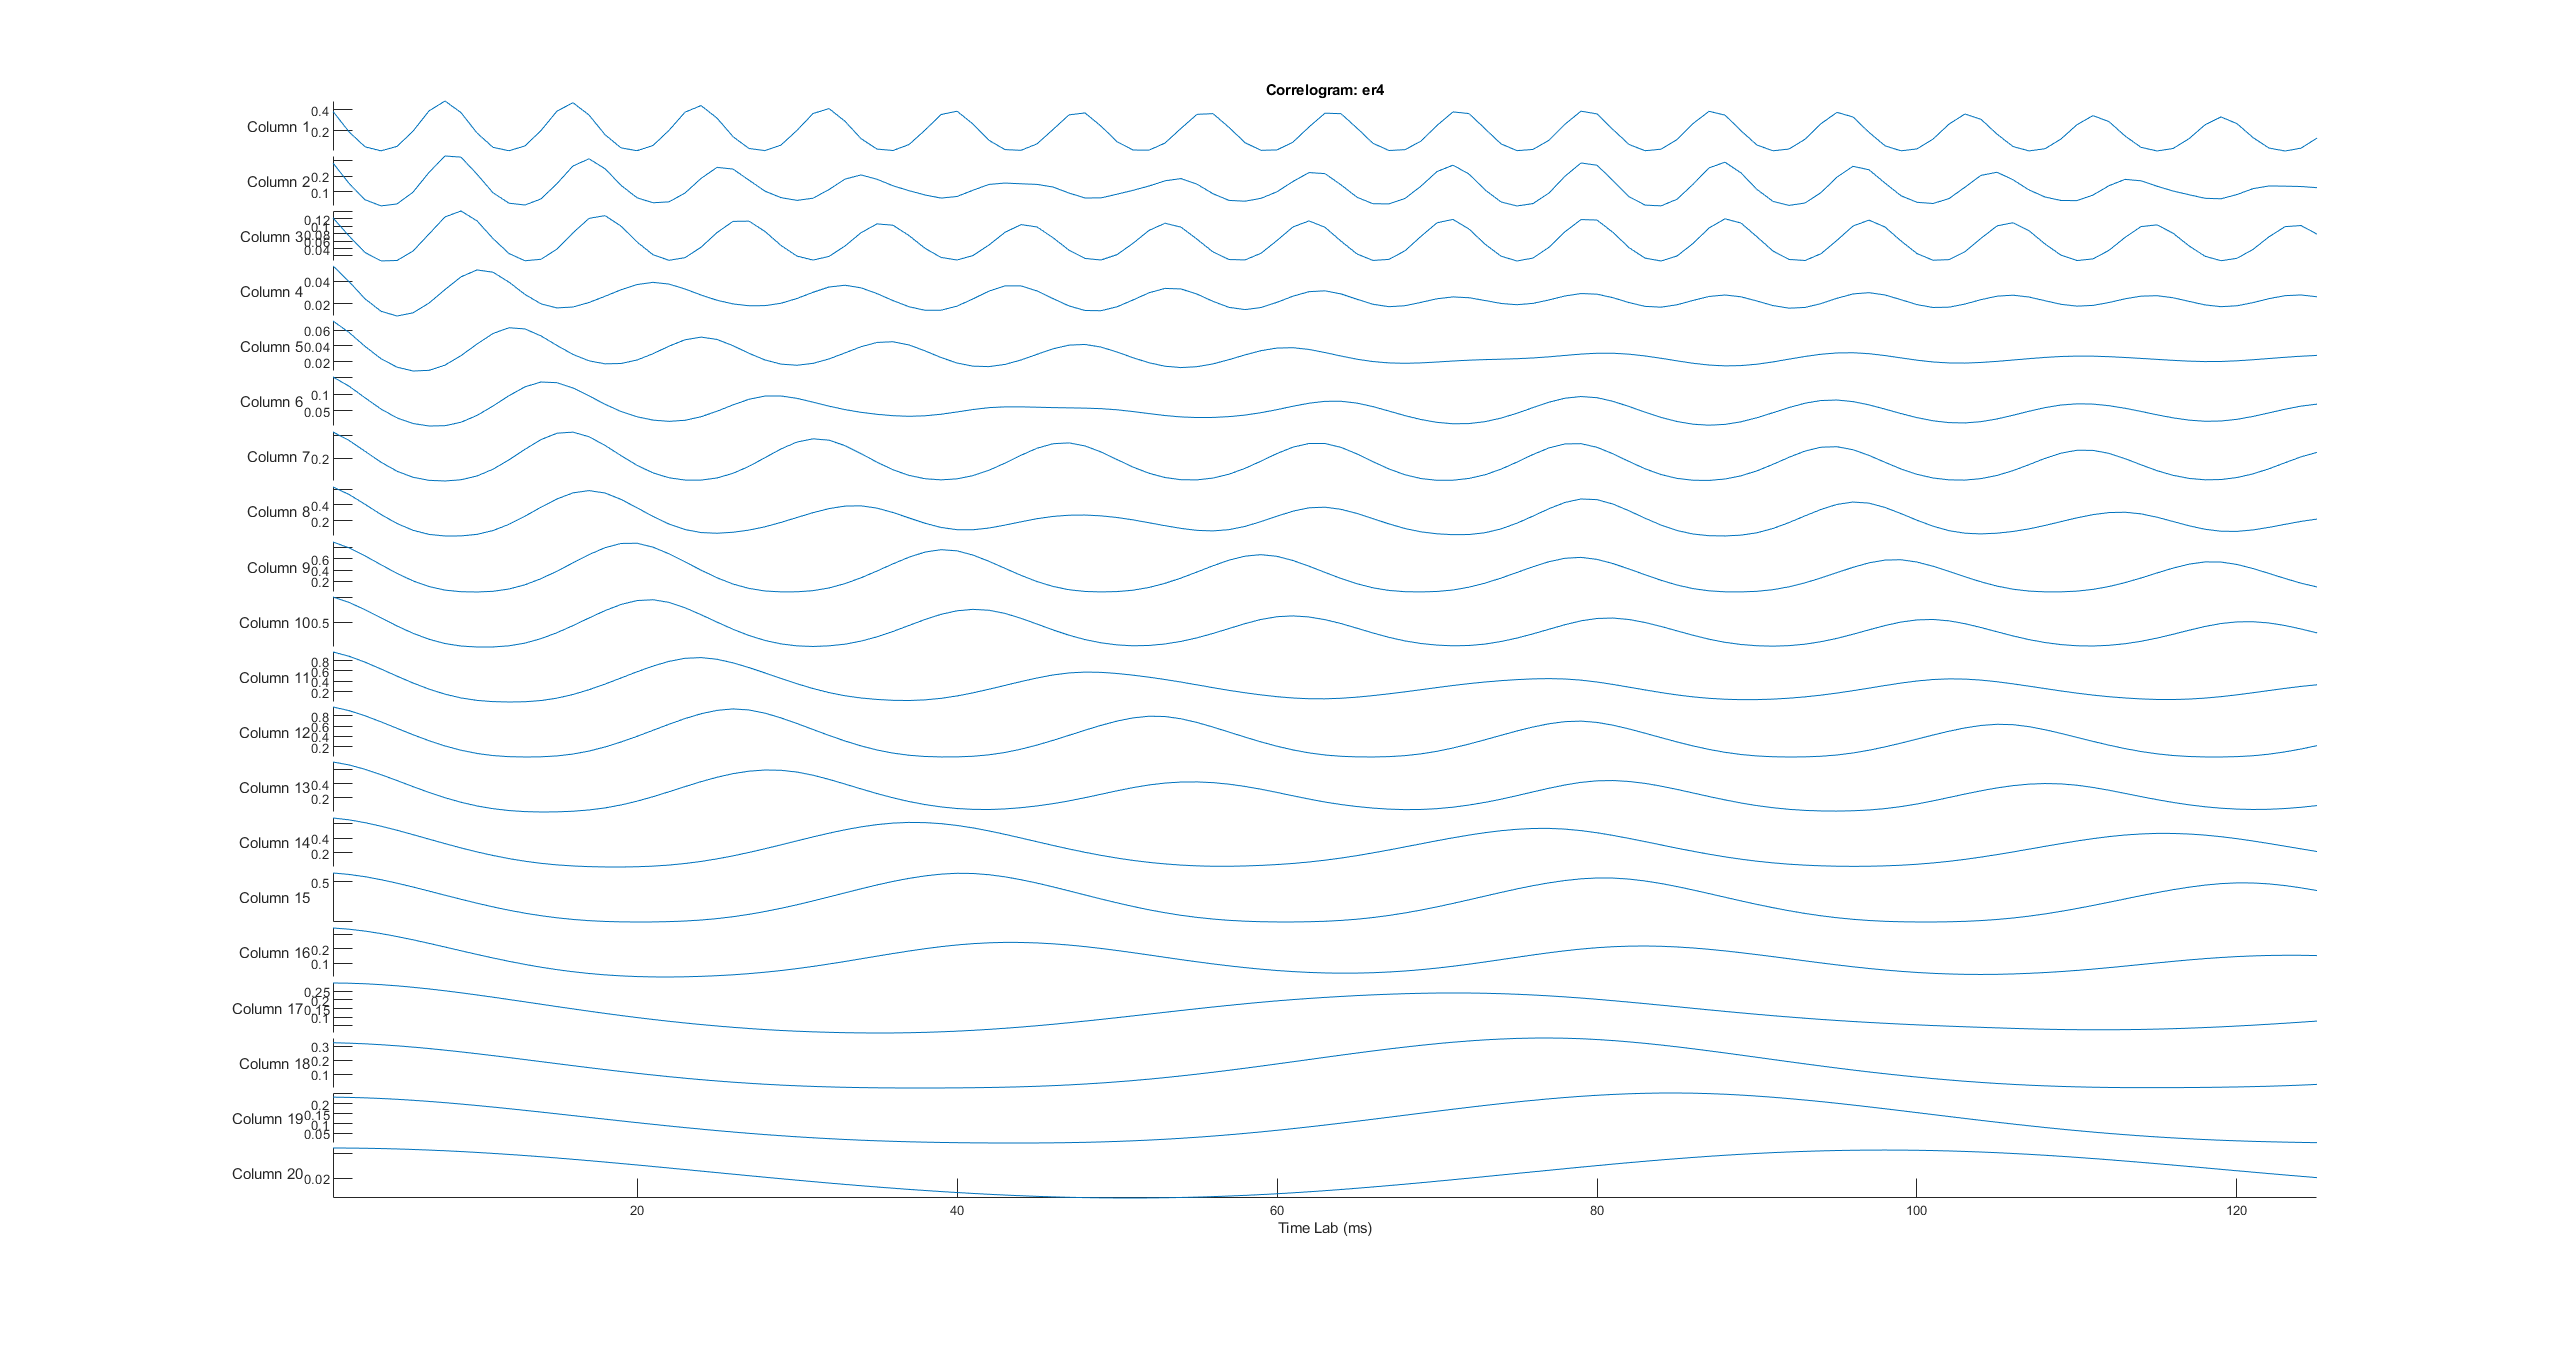
\includegraphics[scale=.25]{er4-correlogram}
  \centering
\end{figure}

While producing the correlogram, I also took the opportunity to create the
summary correlogram. The summary correlogram is produced by accumulating
autocorrelations across channels. As a result, the final graph is a single curve
which contains information that can be used for peak detection. Below is a copy
of the code that produced the correlogram as well as the summary correlogram.

\begin{minted}{matlab}
function [acg, summary] = correlogram(data, MAX_DELAY, CHANNELS, MAX_WINDOW)
    acg = zeros(MAX_DELAY, CHANNELS);
    summary = zeros(MAX_DELAY, 1);
    for channel = 1:CHANNELS
       for delay = 1:MAX_DELAY
           for window = 1:MAX_WINDOW
               acg(delay, channel) = acg(delay, channel) + (
                                     data(channel, window) *
                                     data(channel, window + delay));
           end
           summary(delay, 1) = summary(delay, 1) + acg(delay, channel);
       end
    end
end
\end{minted}

The following images are the summary correlograms generated from the output
of the code above:

\begin{figure}[H]
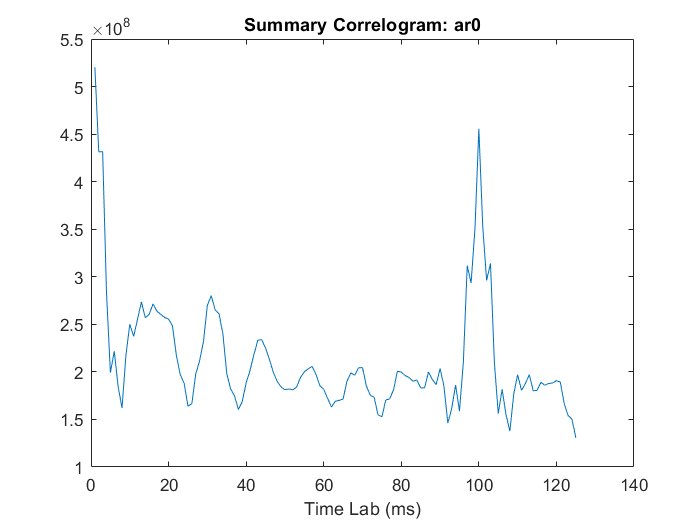
\includegraphics[scale=.75]{ar0-summary-correlogram}
\centering
\end{figure}

\begin{figure}[H]
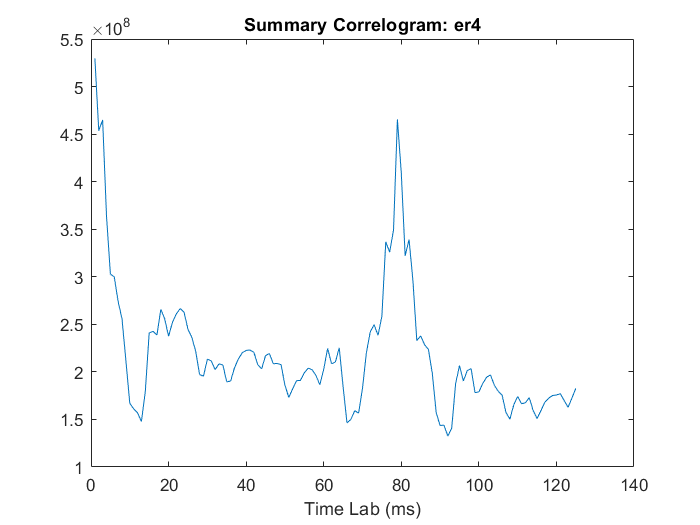
\includegraphics[scale=.75]{er4-summary-correlogram}
\centering
\end{figure}

To perform peak detection, I had to determine safe bounds for searching. After
all, each time step in the lag corresponds to a frequency, and time steps at
0 would constitute a division by 0. Naturally, I wouldn't want to make the
mistake of including values close to 0. Instead, I chose to limit the range
to frequencies between 80 Hz and 222 Hz. These values correspond to time lags
of 125 and 45 respectively.

Finally, all I had to do was find the index of the maximum value between 45 and
125 ms in the summary correlogram. This was accomplished using the max function
in MATLAB which returns both the value and the index of the max value in the
summary correlogram. Using the index, I was able to find the fundamental
frequency through its inverse. Below is the chunk of code I used to perform
fundamental frequency detection:

\begin{minted}{matlab}
function f = fundamental_frequency(SAMPLING_FQ, F0_MIN, F0_MAX, summary)
    starting_bound = int64(SAMPLING_FQ / F0_MAX);
    ending_bound = int64(SAMPLING_FQ / F0_MIN);
    [~, i] = max(summary(starting_bound:ending_bound));
    f = (1.0 / double(i + starting_bound - 1)) * SAMPLING_FQ;
end
\end{minted}

For "ar0.dat", the fundamental frequency was 100 Hz. Meanwhile for "er4.dat",
the fundamental frequency was 126.5823 Hz.

\end{homeworkProblem}

\pagebreak



\end{document}
